\chapter{Nhiệt độ từ entropy và năng lượng}

\lectureoverview{Ban đầu, nhiệt độ xuất hiện như một phép chuyển đổi từ các đơn vị nhiệt kế của con người sang các đơn vị năng lượng vi mô. Sau khi thực hiện phép chuyển đổi tương ứng từ entropy nhiệt động lực học sang entropy thống kê không thứ nguyên, ta mô tả trạng thái cân bằng bằng một họ một tham số các phân bố xác suất. Khi đó, đạo hàm \(dE/dS\) xác định nhiệt độ, và hai định luật đầu tiên cho thấy vì sao chênh lệch nhiệt độ quyết định hướng truyền năng lượng.}

\section{Các hệ số chuyển đổi và các đơn vị do con người đặt ra}

Nhiều hằng số vật lý là các hệ số chuyển đổi. Tốc độ ánh sáng chuyển đổi một khoảng cách thành một thời gian:
\begin{equation}
 t=\frac{x}{c}.
\end{equation}
Nếu khoảng cách và thời gian được đo bằng các đơn vị tương thích, ta có thể đặt \(c=1\). Không có hiệu ứng vật lý nào biến mất; chỉ là hai kiểu phép đo đã được đặt lên cùng một thang chung.

Hằng số Boltzmann có cùng tính chất. Nó chuyển đổi nhiệt độ đọc được trên một nhiệt kế ở quy mô con người thành năng lượng. Tính từ
\emph{quy mô con người} là quan trọng. Những đơn vị như vậy được chọn vì các dụng cụ vĩ mô có thể tạo ra và phân biệt được chúng, chứ không phải vì động lực học vi mô chọn riêng chúng.

Độ Celsius được cố định bằng cách chia khoảng giữa điểm đóng băng và điểm sôi của nước ở áp suất chuẩn thành một trăm phần. Kelvin dùng một độ có cùng kích thước nhưng đặt số 0 tại độ không tuyệt đối. Việc chọn một chất khác, một khoảng khác hoặc độ Fahrenheit sẽ làm thay đổi các con số chứ không làm thay đổi vật lý.

\begin{classroomqa}
\audiencequestion{Thang Fahrenheit đã được xây dựng từ thế kỷ XVII rồi sao?}
\lecturerresponse{Ở đây không cần đến niên đại chính xác. Điểm cốt yếu là mọi thang như vậy đều được thiết kế xoay quanh những nhiệt độ mà con người có thể tạo ra và đo được. Kích thước một độ của chúng là theo quy ước chứ không phải theo vi mô.
\lecturetimestamp{00:01:34--00:01:50}}
\end{classroomqa}

Vào thời các thang đo này được tạo ra, nguồn gốc phân tử của nhiệt chưa thể khảo sát bằng thực nghiệm. Một thay đổi một độ có thể được quan sát bằng nhiệt kế vĩ mô, trong khi năng lượng của một phân tử thì không thể đo được. Vì vậy, việc đặt ra một đơn vị nhiệt độ trước khi người ta biết rằng nhiệt độ về cơ bản là một thang năng lượng là điều tự nhiên.

\section{Vì sao nhiệt độ có đơn vị năng lượng}

Xét một khí đơn nguyên tử loãng. Loãng nghĩa là có thể bỏ qua năng lượng tương tác giữa các phân tử cho mục đích hiện tại. Trong cân bằng nhiệt, nguyên lý phân bố đều gán \(T_{\mathrm K}/2\) nhân với hằng số Boltzmann cho mỗi bậc tự do tịnh tiến có dạng bậc hai. Trong ba chiều không gian,
\begin{equation}
 \left\langle E_{\mathrm{kin}}\right\rangle
 =\frac{3}{2}k_{\mathrm B}T_{\mathrm K}.
 \label{eq:sm2-equipartition-kelvin}
\end{equation}
Hệ số ba đếm chuyển động theo các hướng \(x\), \(y\) và \(z\). Hệ số một phần hai xuất phát từ động năng bậc hai.

Quan hệ này không phải là điều riêng có của một loài phân tử nào. Trong một hỗn hợp helium và oxygen ở trạng thái cân bằng, mọi hạt tịnh tiến tự do đều có cùng động năng trung bình của chuyển động khối tâm, dù các hạt nặng hơn chuyển động chậm hơn. Vì
\begin{equation}
 E_{\mathrm{kin}}=\frac{1}{2}mv^2,
\end{equation}
năng lượng đặc trưng bằng nhau kéo theo \(v\propto m^{-1/2}\).

Ý tưởng ấy có thể được đẩy tới một ví dụ cố ý cực đoan. Treo lơ lửng một quả bóng bowling trong một chất lưu và để toàn bộ hệ đạt đến cân bằng. Các bậc tự do tịnh tiến Brown của nó được chi phối bởi cùng một thang năng lượng như các bậc tự do của một phân tử. Vận tốc của quả bóng nhỏ hơn một cách phi thường vì khối lượng của nó lớn hơn một cách phi thường, nhưng nhiệt độ so sánh các thang năng lượng chứ không phải tốc độ.

Ở nhiệt độ phòng, \(T_{\mathrm K}\) xấp xỉ \(300\,\mathrm K\), trong khi năng lượng của một bậc tự do vi mô tính theo joule thì rất nhỏ. Vì vậy, hệ số chuyển đổi là rất nhỏ:
\begin{equation}
 k_{\mathrm B}\simeq 1.38\times10^{-23}\,
 \mathrm{J\,K^{-1}}.
 \label{eq:sm2-boltzmann-value}
\end{equation}
Quy mô của nó và số Avogadro có liên hệ với nhau chứ không phải chỉ là ngẫu nhiên:
\begin{equation}
 R=N_{\mathrm A}k_{\mathrm B}.
\end{equation}
Hằng số khí \(R\) mô tả một mol, còn \(k_{\mathrm B}\) mô tả thang tương ứng trên mỗi cấu phần vi mô.

Các công thức cơ bản lặp đi lặp lại tổ hợp
\(k_{\mathrm B}T_{\mathrm K}\). Vì vậy, gọn hơn là định nghĩa
\begin{equation}
 T\equiv k_{\mathrm B}T_{\mathrm K}.
 \label{eq:sm2-energy-temperature}
\end{equation}
Từ đây trở đi, \(T\) tự nó có đơn vị năng lượng, và
\eqref{eq:sm2-equipartition-kelvin} trở thành
\begin{equation}
 \left\langle E_{\mathrm{kin}}\right\rangle=\frac{3}{2}T.
 \label{eq:sm2-equipartition-natural}
\end{equation}
Nếu năng lượng được đo bằng joule, nhiệt độ được đo bằng joule. Nếu năng lượng được đo bằng electron volt, nhiệt độ được đo bằng electron volt. Không hề có một đơn vị tự nhiên mới nào mang tên đơn vị nhiệt độ.

\section{Hai quy ước cho entropy}

Phép chuyển đổi tương tự cũng xuất hiện ở phía entropy. Nhiệt động lực học vĩ mô phát triển từ việc phân tích các động cơ nhiệt. Carnot đưa ra lập luận quyết định về động cơ; về sau Clausius đưa vào entropy nhiệt động lực học và ký hiệu
\(S\). Theo ký hiệu dùng ở đây, hãy gọi đại lượng vĩ mô đó là
\(S_{\mathrm C}\). Đơn vị của nó là năng lượng chia cho nhiệt độ theo nhiệt kế,
chẳng hạn joule trên kelvin.

Entropy thống kê là không thứ nguyên. Với một phân bố rời rạc,
\begin{equation}
 S=-\sum_i p_i\log p_i.
 \label{eq:sm2-statistical-entropy}
\end{equation}
Với logarit tự nhiên, một lựa chọn nhị phân đồng xác suất có entropy \(\log2\); với logarit cơ số hai, cùng lượng đó được gọi là một bit. Hai quy ước entropy liên hệ với nhau bởi
\begin{equation}
 S=\frac{S_{\mathrm C}}{k_{\mathrm B}},
 \qquad
 S_{\mathrm C}=k_{\mathrm B}S.
 \label{eq:sm2-entropy-conversion}
\end{equation}
Một giá trị vĩ mô không lớn lắm tính theo \(\mathrm{J\,K^{-1}}\) tương ứng với một entropy không thứ nguyên khổng lồ, vì nó đếm thông tin được phân bố trên một số lượng khổng lồ các cấu phần vi mô.

Các phương trình \eqref{eq:sm2-energy-temperature} và
\eqref{eq:sm2-entropy-conversion} xác lập quy ước được dùng xuyên suốt:
\[
 [T]=[\text{energy}],
 \qquad
 [S]=1.
\]
Hằng số Boltzmann giờ có thể biến mất khỏi các công thức làm việc. Luôn có thể khôi phục nó bằng cách thay \(T\) bằng \(k_{\mathrm B}T_{\mathrm K}\) và
\(S\) bằng \(S_{\mathrm C}/k_{\mathrm B}\).

\begin{classroomqa}
\audiencequestion{Ngoài hệ số \(3/2\), nhiệt độ mới này có đơn giản chỉ là một năng lượng đo bằng joule không?}
\lecturerresponse{Có, nếu joule là đơn vị năng lượng được chọn. Một joule là đơn vị MKS \(\mathrm{kg\,m^2\,s^{-2}}\). Thay vào đó ta cũng có thể dùng electron volt hoặc bất kỳ đơn vị năng lượng nào khác; khi ấy nhiệt độ phải được biểu diễn bằng chính đơn vị đó. Hệ số \(3/2\) thuộc về ví dụ khí lý tưởng, không thuộc về định nghĩa của nhiệt độ.
\lecturetimestamp{00:15:49--00:16:45}}
\end{classroomqa}

\begin{classroomqa}
\audiencequestion{Nếu trên bảng quy định kelvin, vậy \(k_{\mathrm B}\) chẳng phải khi ấy là một hằng số xác định sao?}
\lecturerresponse{Nó là xác định sau khi cả đơn vị nhiệt độ lẫn đơn vị năng lượng đã được chỉ định. Đổi kelvin thành độ Fahrenheit, hoặc joule thành electron volt, thì giá trị số của nó thay đổi. Sự phụ thuộc vào đơn vị đó chính là cách hành xử của một hệ số chuyển đổi.
\lecturetimestamp{00:16:46--00:18:33}}
\end{classroomqa}

\begin{classroomqa}
\audiencequestion{Giá trị số của hằng số Boltzmann có được xác định bằng thực nghiệm không?}
\lecturerresponse{Có. Về mặt lịch sử, việc xác định nó đòi hỏi thông tin vi mô về các nguyên tử và mật độ số của chúng. Boltzmann hiểu quan hệ giữa năng lượng phân tử và nhiệt độ trước khi các đại lượng đó được biết chính xác, cũng như Newton biết vai trò của hằng số hấp dẫn trước khi nó được đo một cách chính xác.
\lecturetimestamp{00:18:46--00:20:00}}
\end{classroomqa}

\section{Cân bằng là một trạng thái thống kê}

Phép chuyển đổi đơn vị vẫn chưa định nghĩa nhiệt độ. Chạm vào một vật nóng đem lại một trực giác sinh học hữu ích, nhưng nhiệt độ là một đại lượng vật lý dẫn xuất được xây dựng từ năng lượng và entropy.

Hãy hình dung một hệ tiếp xúc với một môi trường lớn mà các điều kiện vĩ mô của nó được giữ cố định. Năng lượng có thể truyền qua lại giữa chúng. Nếu ban đầu hệ có quá nhiều năng lượng, trung bình nó mất năng lượng; nếu có quá ít, trung bình nó nhận năng lượng. Trong cân bằng nhiệt, các trao đổi vi mô vẫn tiếp diễn, nhưng không có dòng trung bình ròng theo chiều nào cả.

Gọi \(i\) là nhãn của một trạng thái vi mô chính xác của hệ và gọi \(E_i\) là năng lượng của trạng thái đó. Cân bằng không có nghĩa là hệ cố định ở một trạng thái. Tương tác của nó với môi trường liên tục làm thay đổi vi trạng thái, vì vậy ta gán một xác suất \(P_i\) cho mỗi khả năng. Các hệ thức cơ bản là
\begin{align}
 \sum_i P_i &=1,
 \label{eq:sm2-normalization}\\
 \sum_i P_iE_i &=\overline E,
 \label{eq:sm2-mean-energy}\\
 S&=-\sum_iP_i\log P_i.
 \label{eq:sm2-equilibrium-entropy}
\end{align}
Dấu gạch trên \(\overline E\) nhấn mạnh rằng năng lượng của phân hệ dao động. Một phép đo có thể cho một giá trị và phép đo tiếp theo cho một giá trị khác; các phép đo lặp lại ổn định theo phân bố có giá trị trung bình là
\eqref{eq:sm2-mean-energy}.

\begin{figure}[t]
\centering
\includegraphics[width=0.82\textwidth]{lecture_02_figure_02.png}
\caption{Chuẩn hóa và năng lượng trung bình trên bảng:
\(\sum_iP(i)=1\) và \(\sum_iP(i)E(i)=\langle E\rangle\).}
\lectureframe{00:24:10}
\end{figure}

\section{Một họ được gắn nhãn bằng năng lượng trung bình}

Phân bố cân bằng phụ thuộc mạnh vào năng lượng trung bình. Đặt một nồi nước lên bếp thì \(\overline E\) tăng; đặt nó vào tuyết thì \(\overline E\) giảm. Các xác suất thay đổi theo đó. Vì vậy, cân bằng không nên được xem như một phân bố duy nhất mà như một họ một tham số:
\begin{equation}
 P_i(\overline E).
 \label{eq:sm2-family}
\end{equation}
Mỗi phần tử của họ đều thỏa mãn
\begin{align}
 \sum_iP_i(\overline E)&=1,
 \label{eq:sm2-family-normalization}\\
 \sum_iP_i(\overline E)E_i&=\overline E.
 \label{eq:sm2-family-mean}
\end{align}

\begin{figure}[t]
\centering
\includegraphics[width=0.88\textwidth]{lecture_02_figure_03.png}
\caption{Bước chuyển sang \(P(i,\overline E)\). Các phương trình chuẩn hóa, năng lượng trung bình và entropy ở phần trước vẫn còn hiển thị trong khi họ các phân bố được giới thiệu.}
\lectureframe{00:26:29}
\end{figure}

Đối với một đồ thị sơ đồ, hãy sắp xếp các trạng thái theo thứ tự tăng của \(E_i\). Khi đó trục hoành có thể được đọc hoặc là chỉ số \(i\) hoặc là năng lượng tương ứng. Năng lượng trung bình cao hơn dồn trọng số xác suất về phía các trạng thái nằm xa hơn về bên phải. Mỗi đường cong phải giữ tổng diện tích bằng một.

\begin{figure}[t]
\centering
\includegraphics[width=0.88\textwidth]{lecture_02_figure_04.png}
\caption{Một số phân bố sơ đồ \(P(i,\overline E)\). Các đường cong có trọng số lệch nhiều hơn về bên phải thì có năng lượng trung bình lớn hơn, trong khi mỗi đường vẫn được chuẩn hóa.}
\lectureframe{00:28:40}
\end{figure}

\begin{figure}[t]
\centering
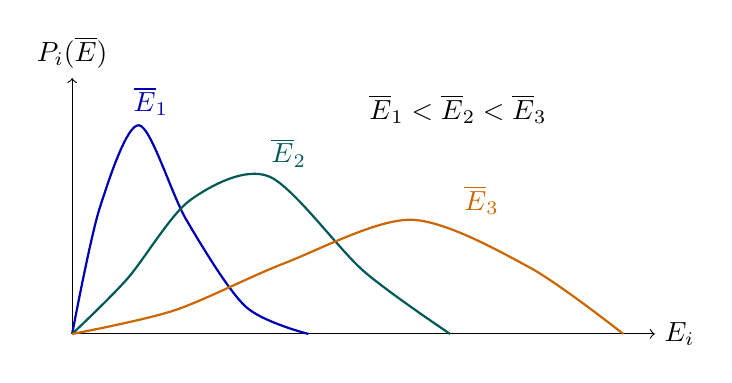
\begin{tikzpicture}[x=1cm,y=1cm]
\draw[->] (0,0) -- (7.4,0) node[right] {$E_i$};
\draw[->] (0,0) -- (0,3.25) node[above] {$P_i(\overline E)$};
\draw[thick,blue!70!black]
  plot[smooth] coordinates {(0,0) (0.35,1.6) (0.85,2.65) (1.45,1.45)
  (2.2,0.35) (3.0,0)};
\draw[thick,teal!70!black]
  plot[smooth] coordinates {(0,0) (0.7,0.7) (1.5,1.7) (2.5,2.0)
  (3.7,0.8) (4.8,0)};
\draw[thick,orange!80!black]
  plot[smooth] coordinates {(0,0) (1.3,0.3) (2.7,0.9) (4.3,1.45)
  (5.8,0.85) (7.0,0)};
\node[blue!70!black] at (1.0,2.95) {\(\overline E_1\)};
\node[teal!70!black] at (2.75,2.3) {\(\overline E_2\)};
\node[orange!80!black] at (5.2,1.7) {\(\overline E_3\)};
\node at (4.9,2.85) {\(\overline E_1<\overline E_2<\overline E_3\)};
\end{tikzpicture}
\caption{Phiên bản được vẽ lại rõ ràng của hình phác trên bảng. Các đường cong không nhất thiết phải có đúng những dạng này; điều duy nhất được dùng là tính chuẩn hóa và thứ tự các năng lượng trung bình của chúng.}
\end{figure}

\begin{classroomqa}
\audiencequestion{Kí hiệu này có mang tính vòng tròn không? Năng lượng trung bình được tính từ phân bố, trong khi phân bố lại được gắn nhãn bằng năng lượng trung bình.}
\lecturerresponse{Hãy bắt đầu với một họ một tham số gồm các phân bố cân bằng được chọn theo thực nghiệm. Mỗi thành viên có một năng lượng trung bình. Nếu các thành viên khác nhau có các năng lượng trung bình khác nhau, thì có thể dùng chính đại lượng đó làm tham số để gọi tên họ. Kí hiệu này chưa suy ra họ ấy; phân bố Boltzmann sẽ cung cấp phép suy ra đó về sau.
\lecturetimestamp{00:28:35--00:29:44}}
\end{classroomqa}

\begin{classroomqa}
\audiencequestion{Vì sao nói năng lượng trung bình thay vì tổng năng lượng?}
\lecturerresponse{Phân hệ đang trao đổi năng lượng với một bể nhiệt, chẳng hạn khí quyển bao quanh một bình chứa khí có các vách thấm nhiệt. Năng lượng tức thời của nó thăng giáng. Nhiều phép đo cho ra một phân bố, và \(\overline E\) là giá trị trung bình của các kết quả đó. Năng lượng của hệ kín lớn hơn gồm phân hệ cộng với bể nhiệt vẫn có thể là cố định.
\lecturetimestamp{00:29:46--00:30:56}}
\end{classroomqa}

\begin{classroomqa}
\audiencequestion{Các vi trạng thái khác nhau có thể có cùng năng lượng không, và các phân bố khác nhau có thể có cùng năng lượng trung bình không?}
\lecturerresponse{Cả hai điều đó đều có thể xảy ra. Bản thân ràng buộc năng lượng trung bình cho phép nhiều phân bố, nên họ cân bằng một tham số đặc biệt ấy đòi hỏi một lập luận vật lý bổ sung. Nguồn gốc của nó và dạng Boltzmann của nó sẽ được suy ra về sau. Việc các vi trạng thái khác nhau có năng lượng bằng nhau là vấn đề riêng, gọi là suy biến.
\lecturetimestamp{00:30:58--00:32:22}}
\end{classroomqa}

\subsection{Nhãn trạng thái, suy biến và tương quan}

Cần tách bạch một số sự phân biệt rất dễ bị nhập nhằng.

Thứ nhất, nhiều phân bố xác suất có thể có cùng một năng lượng trung bình. Họ cân bằng một tham số không thu được chỉ từ riêng ràng buộc năng lượng trung bình. Đó là họ cụ thể được chọn bởi quá trình đạt cân bằng; dạng của nó về sau sẽ được nhận diện là phân bố Boltzmann.

Thứ hai, nhiều vi trạng thái khác nhau có thể có cùng một năng lượng. Điều này được gọi là suy biến. Phần thảo luận trên bảng tạm thời bỏ qua các trường hợp suy biến chính xác để các trạng thái có thể được sắp thứ tự theo năng lượng một cách không nhập nhằng. Trên thực tế, suy biến là phổ biến khi một hệ có đối xứng, nhưng nó không gây ra vấn đề khái niệm nào: giữ lại nhãn trạng thái \(i\), cho phép \(E_i\) nhận các giá trị lặp lại, và cộng trên mọi trạng thái.

Thứ ba, tương quan không phải là một cách gọi khác của suy biến. Tương quan liên quan đến phân bố chung của hai đại lượng ngẫu nhiên và hỏi liệu việc biết một đại lượng có làm thay đổi các xác suất của đại lượng kia hay không. Bản thân các nhãn loại trừ lẫn nhau \(i\) và \(j\) trong một danh sách vi trạng thái không phải là hai biến ngẫu nhiên mà ta đang tính tương quan của chúng.

\begin{classroomqa}
\audiencequestion{Liệu cách xây dựng này có giả định rằng các trạng thái \(i\) khác nhau là độc lập hay không, và nếu hai trong số chúng tương quan với nhau thì sao?}
\lecturerresponse{Một nhãn trạng thái là một giá trị có thể có của một biến ngẫu nhiên vi mô duy nhất. Tính độc lập và tương quan đòi hỏi hai biến có phân bố chung, nên thuật ngữ đó không áp dụng trực tiếp cho hai nhãn thay thế nhau trong danh sách này. Ngược lại, việc các trạng thái khác nhau có cùng năng lượng là một vấn đề về suy biến.
\lecturetimestamp{00:32:23--00:33:22}}
\end{classroomqa}

\begin{classroomqa}
\audiencequestion{Nếu hai trạng thái khác nhau có đúng cùng một năng lượng thì sao?}
\lecturerresponse{Đó là suy biến. Đối với đồ thị đang xét ngay lúc này, ta chấp nhận giả thiết đơn giản hóa rằng không có hai năng lượng nào trùng nhau và sắp các trạng thái theo năng lượng tăng dần. Các công thức xác suất về sau không đòi hỏi giả thiết này; các trạng thái suy biến đơn giản là được đếm riêng.
\lecturetimestamp{00:33:23--00:34:04}}
\end{classroomqa}

\begin{classroomqa}
\audiencequestion{Ý nghĩa của chỉ số \(i\) có tùy ý không?}
\lecturerresponse{Bản thân các trạng thái vi mô không phải là tùy ý: mỗi trạng thái xác định mọi vị trí, xung lượng hoặc dữ liệu khác cần thiết cho một mô tả chính xác. Tên gọi của chúng là tùy ý, nên đối với hình vẽ ta chọn các nhãn theo thứ tự năng lượng tăng dần.
\lecturetimestamp{00:34:06--00:35:15}}
\end{classroomqa}

\section{Entropy trở thành hàm của năng lượng}

Mỗi thành viên của họ cân bằng đều có một entropy. Thay \eqref{eq:sm2-family} vào \eqref{eq:sm2-equilibrium-entropy} ta được
\begin{equation}
 S(\overline E)
 =-\sum_iP_i(\overline E)\log P_i(\overline E).
 \label{eq:sm2-entropy-energy}
\end{equation}
Đây không phải là một hàm phổ quát duy nhất chung cho mọi hệ vật lý. Nó phụ thuộc vào phổ của hệ và vào họ cân bằng của hệ. Tuy nhiên, một khi họ đó đã được xác định thì năng lượng và entropy gắn với nhau: đi dọc theo họ ấy sẽ làm thay đổi cả hai.

Các hệ thông thường thường phân tán xác suất của mình trên nhiều trạng thái hơn khi năng lượng trung bình tăng, nên \(S\) thường tăng theo \(\overline E\). Hiện tại ta giả sử quan hệ này là trơn và khả nghịch cục bộ. Các ngoại lệ là quan trọng, nhưng trường hợp đơn giản làm bộc lộ rõ định nghĩa mà ta cần.

\section{Đạo hàm định nghĩa nhiệt độ}

Hãy đặt một câu hỏi cụ thể: năng lượng trung bình phải thay đổi bao nhiêu để entropy tăng thêm tương ứng với một lựa chọn nhị phân? Trong đơn vị log tự nhiên, độ tăng entropy đó là \(\log2\).

Đối với hai phần tử lân cận trong một họ trơn,
\begin{equation}
 dE=\frac{dE}{dS}\,dS.
 \label{eq:sm2-differential-identity}
\end{equation}
Ở đây phương trình này mới chỉ là quy tắc dây chuyền. Tuy nhiên, hệ số của nó có đúng thứ nguyên và vai trò vật lý mà nhiệt độ phải có.

\begin{definition}
Nhiệt độ, tính theo đơn vị năng lượng, được định nghĩa là
\begin{equation}
 T\equiv\frac{dE}{dS}.
 \label{eq:sm2-temperature-definition}
\end{equation}
Tương đương,
\begin{equation}
 dE=T\,dS,
 \qquad
 dS=\frac{1}{T}\,dE.
 \label{eq:sm2-fundamental-differentials}
\end{equation}
\end{definition}

Nếu xét một biến thiên một bit mà đủ nhỏ,
\begin{equation}
 \Delta E\simeq T\log2.
 \label{eq:sm2-one-bit-energy}
\end{equation}
Việc bám vào một bit chỉ là một cách làm cho đạo hàm trở nên cụ thể. Mọi biến thiên entropy nhỏ đều tuân theo cùng quan hệ cục bộ ấy.

\begin{classroomqa}
\audiencequestion{Vì entropy đã được viết thành \(S(E)\), chẳng phải \(dS/dE\) sẽ là đạo hàm tự nhiên hơn sao?}
\lecturerresponse{Khi quan hệ là khả nghịch cục bộ, cả hai đạo hàm đều chứa cùng một thông tin:
\[
 \frac{dE}{dS}=\left(\frac{dS}{dE}\right)^{-1}.
\]
Theo quy ước, nhiệt độ là \(dE/dS\), còn nhiệt độ nghịch đảo là \(dS/dE=1/T\).
\lecturetimestamp{00:40:24--00:40:54}}
\end{classroomqa}

Ở đây chỉ có một biến nhiệt động lực học thay đổi, nên đạo hàm thường là đủ. Khi thể tích, số hạt, độ từ hóa hoặc các biến khác được phép thay đổi, ta phải dùng đạo hàm riêng và nêu rõ những đại lượng nào được giữ cố định. Định nghĩa hiện tại là lát cắt một biến của hình học nhiệt động lực học tổng quát hơn đó.

\subsection{Vì sao hằng số Boltzmann triệt tiêu}

Hãy tạm quay lại các đơn vị trên nhiệt kế. Dùng
\[
 T=k_{\mathrm B}T_{\mathrm K},
 \qquad
 S=\frac{S_{\mathrm C}}{k_{\mathrm B}},
\]
quan hệ cơ bản trở thành
\begin{align}
 dE
 &=\bigl(k_{\mathrm B}T_{\mathrm K}\bigr)
   d\left(\frac{S_{\mathrm C}}{k_{\mathrm B}}\right)\\
 &=T_{\mathrm K}\,dS_{\mathrm C}.
 \label{eq:sm2-carnot-form}
\end{align}
Một thừa số \(k_{\mathrm B}\) đi vào qua nhiệt độ và thừa số nghịch đảo đi vào qua entropy. Chúng triệt tiêu nhau. Đó là vì sao một giáo trình nhiệt động lực học thông thường có thể viết \eqref{eq:sm2-carnot-form} mà không cần hiển thị hằng số Boltzmann.

\begin{classroomqa}
\audiencequestion{Liệu \(S(E)\) có bắt buộc phải khả nghịch không?}
\lecturerresponse{Không phải lúc nào cũng vậy. Đối với các hệ thông thường trong miền đang xét ở đây, việc tăng năng lượng nhìn chung làm phân bố cân bằng trải rộng ra và làm entropy tăng, nên \(S(E)\) là đơn điệu và \(T>0\). Các hệ có phổ bị chặn có thể cho các phản ví dụ, kể cả những miền mà entropy giảm theo năng lượng và nhiệt độ thống kê là âm. Hiện giờ ta tạm gác các trường hợp đó sang một bên.
\lecturetimestamp{00:44:30--00:45:57}}
\end{classroomqa}

\section{Từ đạo hàm trừu tượng đến nóng và lạnh}

Định nghĩa bằng đạo hàm là phổ quát nhưng vẫn còn trừu tượng. Ta muốn thu lại phát biểu quen thuộc rằng năng lượng chảy từ vật nóng hơn sang vật lạnh hơn. Cảm giác đau khi chạm vào một bề mặt nóng là hiện tượng sinh học; màu sắc và bức xạ phát ra phụ thuộc vào các tính chất của ánh sáng. Một định nghĩa thống kê cũng phải có ý nghĩa đối với một khí lý tưởng hóa ngay cả khi bỏ qua bức xạ.

\begin{classroomqa}
\audiencequestion{Liệu ánh sáng do một vật nóng phát ra có thể cung cấp định nghĩa cơ bản của nhiệt độ không?}
\lecturerresponse{Bức xạ là một nhiệt kế hữu ích, nhưng nó đưa vật lý của ánh sáng vào. Cơ học thống kê phải định nghĩa nhiệt độ cho các hệ như một hộp khí mà không dựa vào các tính chất quang học. Chiều trao đổi năng lượng là tiêu chuẩn tổng quát hơn.
\lecturetimestamp{00:46:42--00:47:20}}
\end{classroomqa}

Chuẩn bị hai hệ \(A\) và \(B\), ban đầu mỗi hệ ở trạng thái cân bằng riêng của nó, với các nhiệt độ \(T_A\) và \(T_B\). Ban đầu chúng cách ly với nhau. Sau đó nối chúng bằng một tiếp xúc nhiệt yếu: \emph{ống mỏng} cho phép những lượng năng lượng nhỏ truyền qua lại mà không làm mất tính riêng biệt của bất kỳ phân hệ nào.

\begin{figure}[t]
\centering
\includegraphics[width=0.88\textwidth]{lecture_02_figure_05.png}
\caption{Hai hệ \(A\) và \(B\) được chuẩn bị riêng rẽ, được đặc trưng bởi các nhiệt độ \(T_A\) và \(T_B\), ngay trước khi xét tiếp xúc nhiệt yếu.}
\lectureframe{00:48:55}
\end{figure}

\begin{figure}[t]
\centering
\begin{tikzpicture}[>=Stealth]
\draw[rounded corners,thick,fill=blue!6] (0,0) rectangle (2.6,2.4);
\draw[rounded corners,thick,fill=orange!8] (5.4,0) rectangle (8,2.4);
\draw[thick] (2.6,1.35) -- (5.4,1.35);
\draw[thick] (2.6,1.05) -- (5.4,1.05);
\draw[<->,very thick] (3.15,1.2) -- (4.85,1.2)
  node[midway,above] {\(\delta E\)};
\node at (1.3,1.45) {\Large \(A\)};
\node at (6.7,1.45) {\Large \(B\)};
\node at (1.3,0.65) {\(T_A,S_A,E_A\)};
\node at (6.7,0.65) {\(T_B,S_B,E_B\)};
\node at (4,0.35) {\small weak thermal contact};
\end{tikzpicture}
\caption{Năng lượng thăng giáng qua tiếp xúc yếu trong khi hệ kết hợp vẫn cô lập.}
\end{figure}

Giả sử, không mất tính tổng quát,
\begin{equation}
 T_B>T_A.
 \label{eq:sm2-temperature-order}
\end{equation}
Kinh nghiệm cho thấy \(B\) phải mất năng lượng còn \(A\) phải nhận năng lượng. Ba thực tế biến kỳ vọng đó thành một phép tính.

\subsection{Tính cộng của entropy}

Đối với hai phân hệ ghép yếu mà các khả năng vi mô kết hợp độc lập với nhau, số khả năng chung được nhân với nhau:
\[
 W_{AB}=W_AW_B.
\]
Entropy có tính lôgarit, nên
\begin{equation}
 S_{\mathrm{tot}}=S_A+S_B.
 \label{eq:sm2-entropy-additivity}
\end{equation}
Kết quả ấy cũng suy ra trực tiếp từ entropy Shannon của một phân bố tích.

\begin{classroomqa}
\classquestion{Vì sao entropy của hệ kết hợp lại có tính cộng?}
\lecturerresponse{Bởi vì số khả năng cơ sở được nhân với nhau còn entropy thì lấy lôgarit:
\(\log(W_AW_B)=\log W_A+\log W_B\). Tương tác yếu chính là điều cho phép mô tả theo phân hệ và dạng cộng bậc đầu này.
\lecturetimestamp{00:51:06--00:52:03}}
\end{classroomqa}

\subsection{Định luật thứ nhất và thứ hai}

Hệ kết hợp là cô lập, nên năng lượng trao đổi ở bên trong được bảo toàn:
\begin{equation}
 dE_A+dE_B=0,
 \qquad
 dE_B=-dE_A.
 \label{eq:sm2-first-law}
\end{equation}
Đây là định luật thứ nhất trong thí nghiệm đang xét.

Ở đây, định luật thứ hai được lấy làm một tiên đề, sẽ được giải thích sâu hơn về sau.
Khi các hệ đã nối với nhau thư giãn về phía trạng thái cân bằng mới của chúng,
\begin{equation}
 dS_{\mathrm{tot}}=dS_A+dS_B\geq0.
 \label{eq:sm2-second-law}
\end{equation}
Bất đẳng thức nghiêm mô tả sự thư giãn tự phát từ trạng thái ngoài cân bằng; dấu bằng đúng tại cân bằng đối với biến thiên thuận nghịch bậc một.

Cuối cùng, định nghĩa nhiệt độ áp dụng cho từng phân hệ:
\begin{equation}
 dE_A=T_A\,dS_A,
 \qquad
 dE_B=T_B\,dS_B.
 \label{eq:sm2-two-temperatures}
\end{equation}

\begin{figure}[H]
\centering
\includegraphics[width=0.88\textwidth]{lecture_02_figure_06.png}
\caption{Hai hệ thức của hai phân hệ \(dE_A=T_A\,dS_A\) và \(dE_B=T_B\,dS_B\) ở phần kết của lập luận trên bảng.}
\lectureframe{00:54:00}
\end{figure}

\subsection{Dấu của dòng năng lượng}

Những phương trình này đã xác định hướng của sự truyền ròng. Thay \(dS_A=dE_A/T_A\), \(dS_B=dE_B/T_B\), và
\eqref{eq:sm2-first-law} vào \eqref{eq:sm2-second-law}:
\begin{align}
 dS_{\mathrm{tot}}
 &=\frac{dE_A}{T_A}+\frac{dE_B}{T_B}\\
 &=dE_A\left(\frac{1}{T_A}-\frac{1}{T_B}\right)\geq0.
 \label{eq:sm2-flow-sign}
\end{align}
Nếu \(T_B>T_A>0\), thì
\[
 \frac{1}{T_A}-\frac{1}{T_B}>0.
\]
Do đó, phương trình \eqref{eq:sm2-flow-sign} đòi hỏi
\[
 dE_A>0,
 \qquad
 dE_B<0.
\]
Phân hệ lạnh hơn \(A\) nhận năng lượng, còn phân hệ nóng hơn \(B\) mất năng lượng.
Khi \(T_A=T_B\), biến thiên entropy bậc một không chỉ ra hướng ưu tiên nào, và các trao đổi vi mô cân bằng nhau nên dòng ròng bằng không. Vì vậy, đạo hàm trừu tượng \(T=dE/dS\) tái hiện sự phân biệt theo thao tác giữa nóng và lạnh.
